\chapter{ПРОЕКТИРОВАНИЕ ИГРОВОЙ СРЕДЫ И ОБУЧАЮЩЕГО АГЕНТА}

\section{Требования к игровой среде}

Среда должна решать сразу две задачи. С одной стороны, она должна правильно реализовывать саму игру: движение змейки, появление пищи, рост длины и завершение партии при столкновении. С другой стороны, она должна быть удобной для обучения агента: возвращать состояние, принимать действие и выдавать численную награду.

В проекте используется поле размером $20 \times 20$ клеток. Змейка начинает движение из центра поля и сначала направлена вправо. Такое начальное положение удобно, потому что оно симметрично и не даёт преимущества какой-то одной стороне поля.

\begin{table}[H]
    \centering
    \caption{Основные параметры игровой среды и обучения}
    \begin{tabularx}{\textwidth}{>{\raggedright\arraybackslash}p{0.3\textwidth} >{\raggedright\arraybackslash}p{0.18\textwidth} X}
        \toprule
        Параметр & Значение & Назначение \\
        \midrule
        Размер поля & $20 \times 20$ & Количество клеток по горизонтали и вертикали \\
        Размер клетки & 24 px & Масштаб визуализации в окне Pygame \\
        FOOD\_REWARD & 10.0 & Награда за поедание пищи \\
        COLLISION\_PENALTY & -10.0 & Штраф за столкновение \\
        STEP\_PENALTY & -0.1 & Небольшой штраф за каждый ход \\
        ALPHA & 0.1 & Скорость обновления Q-оценок \\
        GAMMA & 0.9 & Учёт будущих вознаграждений \\
        EPSILON & 1.0 & Начальная интенсивность исследования \\
        EPSILON\_DECAY & 0.995 & Множитель снижения $\varepsilon$ \\
        EPSILON\_MIN & 0.05 & Нижняя граница $\varepsilon$ \\
        TRAIN\_EPISODES & 300 & Базовое число эпизодов обучения \\
        \bottomrule
    \end{tabularx}
\end{table}

\section{Формирование пространства состояний}

Одним из главных решений в проекте стал выбор состояния агента. Если хранить все координаты змейки и еды, число состояний быстро станет слишком большим. Поэтому в работе используется более компактный вариант --- вектор из 11 бинарных признаков.

В этот вектор входят признаки опасности при движении прямо, влево и вправо, текущее направление змейки и положение пищи относительно головы. Такой набор даёт агенту ту информацию, которая действительно нужна для выбора следующего хода, и при этом не делает модель слишком сложной.

Такой подход важен не только для удобства реализации, но и для самой логики обучения. Агенту не обязательно знать полную геометрию поля в каждый момент времени, если для принятия ближайшего решения ему достаточно понимать три вещи: есть ли опасность рядом, куда он сейчас движется и с какой стороны находится цель. За счёт этого состояние получается компактным и хорошо подходит для табличного Q-learning.

Ещё одно достоинство такого описания состоит в том, что оно делает поведение агента более обобщаемым. Разные игровые ситуации, которые с точки зрения координат выглядят по-разному, могут совпадать по смыслу: например, во всех них еда находится справа, а впереди есть опасность. В табличном методе это особенно полезно, потому что позволяет использовать один и тот же набор оценок для типовых игровых шаблонов.

\begin{table}[H]
    \centering
    \caption{Состав вектора состояния среды}
    \begin{tabularx}{\textwidth}{>{\centering\arraybackslash}p{0.08\textwidth} >{\raggedright\arraybackslash}p{0.26\textwidth} X}
        \toprule
        № & Признак & Смысл \\
        \midrule
        1 & danger\_straight & Столкновение при движении прямо \\
        2 & danger\_left & Столкновение при повороте влево \\
        3 & danger\_right & Столкновение при повороте вправо \\
        4 & dir\_up & Текущая ориентация вверх \\
        5 & dir\_down & Текущая ориентация вниз \\
        6 & dir\_left & Текущая ориентация влево \\
        7 & dir\_right & Текущая ориентация вправо \\
        8 & food\_left & Пища расположена левее головы \\
        9 & food\_right & Пища расположена правее головы \\
        10 & food\_up & Пища расположена выше головы \\
        11 & food\_down & Пища расположена ниже головы \\
        \bottomrule
    \end{tabularx}
\end{table}

\section{Множество действий и проектирование функции награды}

Вместо абсолютных направлений в проекте используются относительные действия: идти прямо, повернуть влево и повернуть вправо. Это упрощает обучение, потому что агент выбирает действие относительно своего текущего движения, а не относительно экрана.

Награда построена так, чтобы агенту было выгодно искать пищу и избегать бесполезных ходов. За поедание пищи он получает 10.0, за столкновение --- штраф -10.0, а за обычный шаг --- небольшой штраф -0.1. За счёт этого агент учится не просто долго жить, а двигаться к цели.

Выбор относительных действий особенно важен с точки зрения обучения. Если бы агент использовал абсолютные команды вроде <<вверх>>, <<вниз>>, <<влево>> и <<вправо>>, ему пришлось бы отдельно учиться похожим ситуациям для разных текущих направлений движения. Относительная схема уменьшает эту избыточность: действие <<повернуть влево>> имеет один и тот же смысл независимо от того, куда змейка была направлена до этого. Это делает пространство действий меньше и помогает агенту быстрее накапливать полезный опыт.

Функция награды тоже играет ключевую роль. Положительная награда за пищу даёт агенту явную цель. Штраф за столкновение показывает, какие ситуации являются критически плохими. Небольшой штраф за обычный шаг нужен для того, чтобы агент не выбирал бесконечное безопасное движение по кругу, которое не приводит к росту счёта. Иначе в задаче могла бы появиться стратегия, при которой агент долго избегает смерти, но почти не решает основную задачу.

С точки зрения проектирования это означает, что награда задаёт само понятие <<хорошего поведения>>. В данной работе хорошей считается стратегия, которая одновременно избегает столкновений, движется к пище и не тратит слишком много лишних шагов. Именно такой баланс и был заложен в систему вознаграждений.

\section{Архитектура программной системы}

Программа разбита на несколько модулей. Файл \texttt{game.py} отвечает за игровую механику, \texttt{env.py} превращает игру в среду для обучения, \texttt{agent.py} содержит Q-learning агента, \texttt{train.py} управляет обучением, \texttt{render.py} отвечает за визуализацию, а \texttt{main.py} запускает нужный режим работы.

\begin{figure}[H]
    \centering
    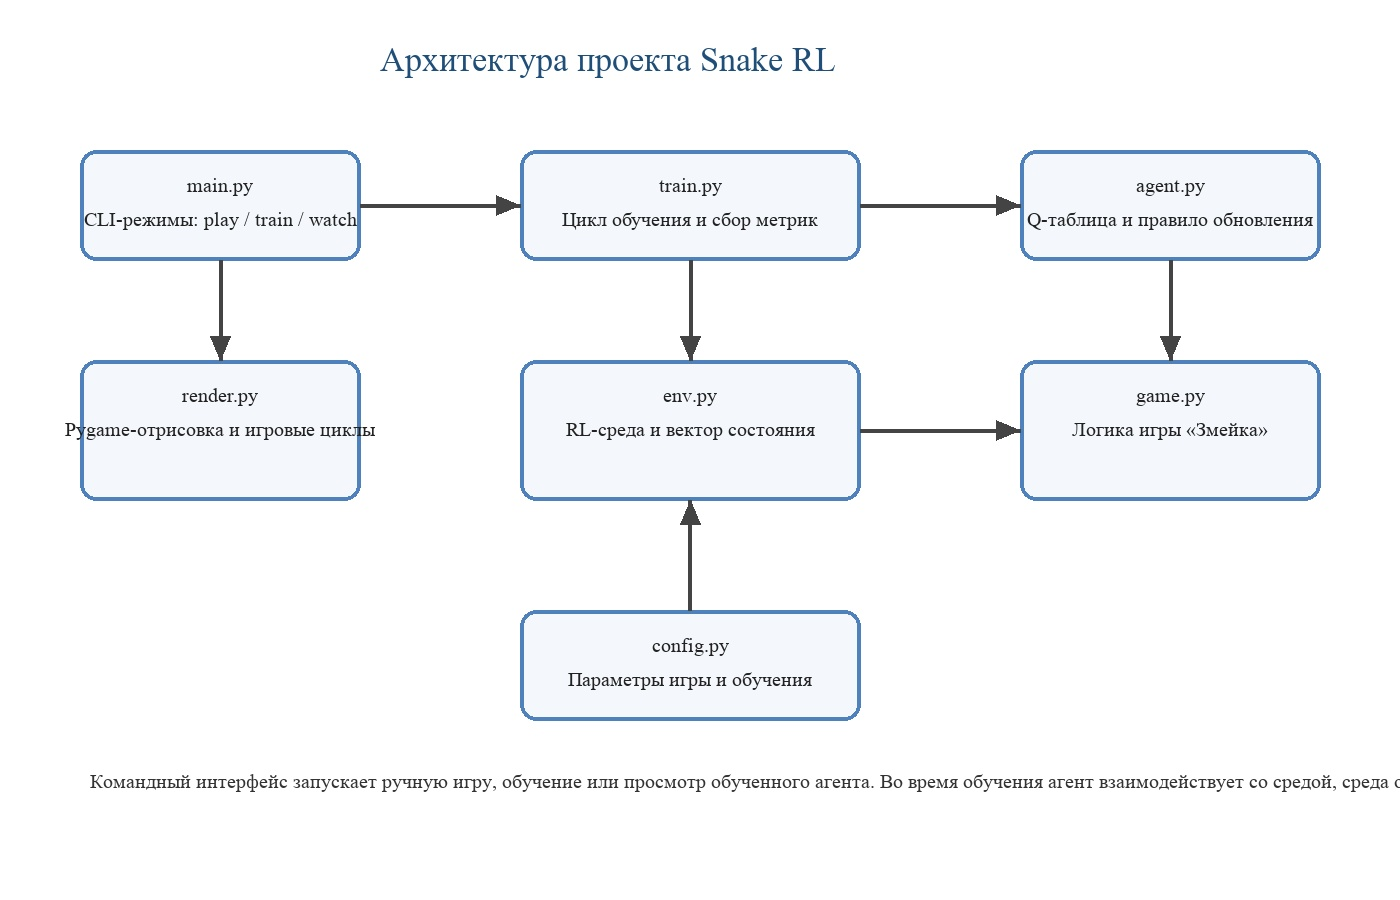
\includegraphics[width=0.92\textwidth]{images/architecture.jpg}
    \caption{Структурная схема взаимодействия модулей проекта}
\end{figure}

Такое разбиение делает проект более понятным и удобным для доработки. Игровую логику, обучение и интерфейс можно рассматривать как отдельные части системы.

Кроме того, такая архитектура удобна и для анализа результатов. Если агент обучается плохо, можно отдельно проверять, правильно ли работает игровая логика, корректно ли формируется состояние, верно ли считается награда и не ошибается ли модуль выбора действия. Это особенно важно в учебном проекте, где цель состоит не только в получении работающей программы, но и в понимании того, как взаимодействуют все её части.
